\newcommand{\mvec}[1]{\mathbf{#1}}
\newcommand{\mvecx}[1]{\mathbf{#1}_x}
\newcommand{\mvecy}[1]{\mathbf{#1}_y}
\newcommand{\mvecz}[1]{\mathbf{#1}_z}
\newcommand{\mvecw}[1]{\mathbf{#1}_w}
\newcommand{\mmat}[1]{\mathbf{#1}}
\newcommand{\transpose}[1]{#1^{\mathsf{T}}}
\newcommand{\inverse}[1]{#1^{\mathsf{-1}}}
\newcommand{\normalise}[1]{\frac{#1}{\norm{#1}}}

\DeclarePairedDelimiter\abs{\lvert}{\rvert}
\DeclarePairedDelimiter\norm{\lVert}{\rVert}

%\renewcommand\Re{\operatorname{Re}}
%\renewcommand\Im{\operatorname{Im}}

\renewcommand{\Re}{\mathcal{R}}
\renewcommand{\Im}{\mathcal{I}} 

\begin{table}[b]
\begin{tabularx}{\textwidth}{X | X X | X X }
 %\hline
  \cline{2-5}
  & \multicolumn{2}{c}{Period Band Range (sec)} \vline & \multicolumn{2}{c}{Frequency Band Range (Hz)} \\
  \hline
  Wave Type & Start & End & Start & End \\
 \hline
  Capillary    & $0$                & $1\times10^{-1}$   & $\infty$            & $1\times10^1$ \\
  Ultragravity & $1\times10^{-1}$   & $1\times10^{0}$    & $1\times10^1$       & $1\times10^0$ \\
  Gravity      & $1\times10^{0}$    & $3\times10^{1}$    & $1\times10^0$       & $3.33\times10^{-2}$ \\
  Infragravity & $3\times10^{1}$    & $3\times10^{2}$    & $3.33\times10^{-2}$ & $3.33\times10^{-3}$ \\
  Long Period  & $3\times10^{2}$    & $8.64\times10^{4}$ & $3.33\times10^{-3}$ & $1.16\times10^{-5}$ \\
  Transtidal   & $8.64\times10^{4}$ & $\infty$           & $1.16\times10^{-5}$ & $0$
\end{tabularx}
\caption{A classification of ocean surface waves by period and frequency.}
\label{tab:ocean_wave_period}
\end{table}

Ocean surface waves are generated by different kinds of forces, such as storms, earthquakes,
the gravity of sun and moon, but with~\emph{wind} being the most prominent one.
Table~\ref{tab:ocean_wave_period} gives a compact overview of different kinds of ocean surface waves
classified by frequency. Figure~\ref{fig:surface_waves_energy}, inspired by Munk~\cite{article:munkorigin}
and Kinsman~\cite{book:kinsman2002wind}, on the other hand, pictures the forces influencing the different kinds of ocean waves.\\

Because ocean surface waves are generated and propagate at the interface between the atmosphere
and the ocean, where the restoring force of gravity is in effect, they are classified as~\emph{surface gravity waves}.
Moreover, since wind blowing over a vast stretch of the air-sea interface is the main force to generate waves on
the ocean surface, this kind of waves are called~\emph{wind generated waves}, or in short,~\emph{wind waves}.
Wind waves on the ocean surface represent gravity waves, while e.g. tsunamis and ocean tides do not.\\

The process behind surface gravity waves is a simple one - the moment a fluid element at the interface is displaced, gravity
will try to restore it to equilibrium which results in oscillation of said fluid element. We mentioned before
that wind is the most prominent force causing displacement on the water surface. As it blows, it causes pressure and friction
forces which perturb the water surface's equilibrium. Therefore, the combination of wind transferring energy from the air
to the water and gravitational acceleration cause the formation of waves on the water surface.\\

In order to be able to model the surface of such an intricate fluid system as the ocean, one has to reduce complexity.
Research fields such as ocean engineering or coastal engineering employ the~\emph{Airy wave theory}\cite{book:airy1845tides}
to model the properties of the sea. Airy wave theory, also known as~\emph{linear wave theory}, describes the propagation of
gravity waves on the surface of a homogeneous fluid with a set of~\emph{linear} equations. These equations give
a decent approximation of the wave dynamics and kinematics with enough accuracy to model the state of the sea over a
limited amount of time.

\begin{figure}[tb]
	\centering
	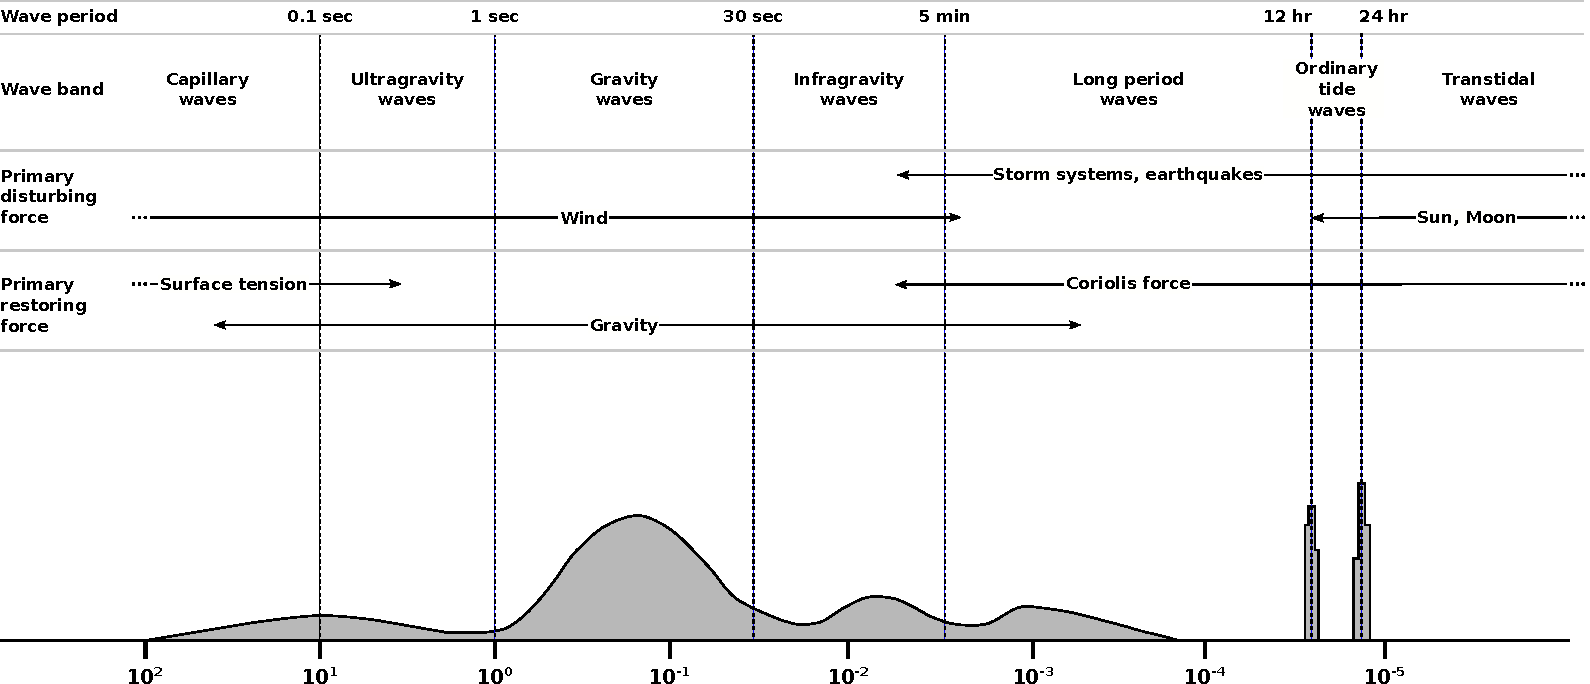
\includegraphics[width=\textwidth]{figures/SurfaceWavesEnergy}
	\caption{A tentative overview of which forces influence which wave band, as well as the relative amount of energy
each wave band contains.}
	\label{fig:surface_waves_energy}
\end{figure}

\section{Linear Theory of Ocean Surface Waves}
\label{sec:linear_theory_ocean_waves}
Linear wave theory makes a set of assumptions about the properties of the fluid, such as its viscosity,
compressibility and curl. Because fluid mechanics and fluid dynamics, associated fluid properties, and the derivation
of the linear wave theory go beyond the scope of this thesis, we will refer the interested reader
to Airy~\cite{book:airy1845tides}, Batchelor~\cite{book:batchelor2000introduction}
and Kinsman~\cite{book:kinsman2002wind}, which provide a good starting point for in-depth information.\\

\emph{But} we will mention two core assumptions of the linear wave theory which are easy to picture:
\begin{itemize}
 \item The water body has a uniform mean depth.
 \item The wave amplitudes are small in relation to the size of the water body.
\end{itemize}
Suppose we observe an idealized ocean in which exactly one sine wave is travelling constantly.
The parameters defining the sine wave - amplitude, frequency, length and direction - are all fixed.
To simplify the mathematics we assume a two-dimensional ocean, with one
dimension representing the wave's direction of travel and the  other the wave's
vertical displacement. With these assumptions we can describe surface elevation
as a sinusoid
%
\begin{equation}
\label{eq:sinusoid}
 \eta(x, t) = A\cos(kx - \omega t)\\
\end{equation}
with
\begin{align}
 k &= \frac{2\pi}{\lambda} & \omega &= 2\pi f & f &= \frac{1}{T}
\end{align}
%
where $A$ is the amplitude, $k$ is called the~\emph{wave number},~$x$ is the horizontal position,
$\omega$ is the~\emph{wave frequency} in radians per second,~$t$ represents the time,
$\lambda$ is the~\emph{wave length},~$f$ is the~\emph{wave frequency} in Hertz (Hz) and~$T$
is the wave period in seconds.\\

\begin{figure}[b]
	\centering
	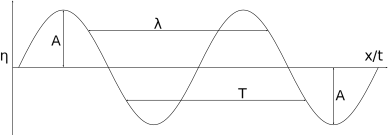
\includegraphics[width=\textwidth]{figures/sinusoid}
	\caption{Sample figure}
	\label{fig:sinusoid}
\end{figure}
%
We may picture Equation~\ref{eq:sinusoid} in an easy way if we either focus on a fixed position $x$
or a fixed point in time $t$, see Figure~\ref{fig:sinusoid}. If we assume a fixed position, we can
see the surface elevation evolve through time at that position. On the other hand, if we assume a fixed
point in time, we can observe surface elevation at all positions at that specific time.
The wave's high point is called a~\emph{crest}, its low point a~\emph{trough}. Because surface elevation
is described by a cosinus function, all crests and all troughs will have the
same elevation. Another effect of the cosinus function is that the surface
elevation is limited by the amplitude $A$. We will call the difference in
elevation between crest and trough the~\emph{wave height}. It is obvious that we
can define wave height $H$ as
\begin{equation}
 H = 2A
\end{equation}
\\

\subsection{Phase Velocity}
\label{sec:phase_velocity}
In linear wave theory, the rate at which a particular phase of a wave propagates in space is called
the~\emph{phase velocity}. The phase velocity is a vector and has an associated direction,
the \emph{phase speed} on the other hand refers only to the magnitude of the phase velocity.
The most comprehensible example of phase speed is the rate of propagation of the wave crest.
During one wave period $T$ the wave crest travels a distance equal to the wave length $\lambda$.
We may generalize this to other phases than the wave crest - given a constant phase
\begin{equation}
  kx - \omega t = const
\end{equation}
the surface elevation $\eta$ will always be the same. We rewrite the term to
\begin{equation}
  x = \frac{\omega}{k}t + \frac{const}{k}
\end{equation}
which gives us all positions $x$ the wave has the same value at. These positions are time dependent,
differentiation gives us phase speed $c$:
\begin{equation}
  c = \frac{\mathrm dx}{\mathrm dt} = \frac{\lambda}{T} = \frac{\omega}{k}
\end{equation}

\subsection{The Dispersion Relation}
\label{sec:dispersion_relation}

In the context of water surface waves,~\emph{dispersion} refers to~\emph{frequency dispersion}, which describes
the effect of waves at different wavelengths travelling at different phase speeds. We have seen that
phase speed $c = \frac{\lambda}{T}$ involves wave length and frequency, and alternatively $c = \frac{\omega}{k}$
which includes angular frequency and wave number. We focus on the latter formulation for phase speed, because
linear wave theory defines a functional relationship between the two factors involved:
%therefore we will start with the functional relationship
%between angular frequency~$\omega$ and wave number~$k$ as defined by linear wave theory:
\begin{equation}
\label{eq:dispersion_relation}
 \omega^2 = gk\tanh(kd)
\end{equation}
%
where $g$ is the acceleration of earth's gravity and $d$ is the water depth. Equation~\ref{eq:dispersion_relation}
is called the~\emph{dispersion relation}.\\

There exist two useful approximations of Equation~\ref{eq:dispersion_relation} which do not involve the $\tanh$ term:
\begin{itemize}
 \item \emph{Shallow water approximation} - the water depth $d$ is much smaller than the wave length $\lambda$.
 Assume $d \ll \lambda$, then $0 \leq kd \ll 1$ and $\tanh(kd) \approx kd$.
 \item \emph{Deep water approximation} - the water depth $d$ is much larger than the wave length $\lambda$.
 Assume $d \gg \lambda$, then $kd \gg 1$ and $\tanh(kd) \approx 1$.
\end{itemize}
%
The reduced dispersion relations are as follows:
\begin{align}
 \omega^2 & = gk^2d && \text{with} & d &< \frac{\lambda}{20}  && \text{Shallow water dispersion relation}\\
 \omega^2 & = gk    && \text{with} & d &> \frac{\lambda}{2} && \text{Deep water dispersion relation}
\end{align}
%
Given the dispersion relation approximations for shallow and deep water, the corresponding
phase speeds are:
\begin{align}
 \label{eq:phase_speed_shallow_water} c &= \sqrt{gd} && \text{Shallow water phase speed}\\
  \label{eq:phase_speed_deep_water}   c &= \sqrt{\frac{g}{k}} = \frac{g}{\omega} && \text{Deep water phase speed}
\end{align}
%
According to Equation~\ref{eq:phase_speed_shallow_water}, in shallow water phase speed depends exclusively
on water depth and gravitational acceleration, there is no connection to wave length or frequency.
We may conclude that waves with different wave lengths travel with the same phase speed, it follows that
~\emph{shallow water is not dispersive}. Phase speed in deep water, on the other hand,
does not relate to water depth, but to wave length and frequency, which makes~\emph{deep water dispersive}.
We can expand Equation~\ref{eq:phase_speed_deep_water} to:
%
\begin{equation}
\label{eq:phase_speed_deep_water_l}
 c = \sqrt{\frac{g\lambda}{2\pi}} = \frac{gT}{2\pi}
\end{equation}
%
Looking at Equation~\ref{eq:phase_speed_deep_water_l} we can conclude that phase speed in deep water increases
with wave length $\lambda$ ~\emph{and} with wave period $T$. Waves in deep water with large wavelengths/periods
travel faster than those with smaller ones.
%
\subsection{Three Dimensional Wave}
Until now we were discussing a two dimensional ocean defined by exactly one sinus wave. As a first
step to get to a more realistic ocean surface representation we will extend equation~\ref{eq:sinusoid}
to form a wave in three dimensional space. In contrast to equation~\ref{eq:sinusoid}, where the wave's
travelling direction is fixed, the wave has to be able to travel in an arbitrary direction on a plane.
Moreover, we need to handle two dimensional input positions. The sinusoid describing surface elevation
in three dimensional space is defined as follows:
\begin{equation}
\label{eq:sinusoid_3d}
 \eta(\mvec{x}, t) = A\cos(\transpose{\mvec{k}}\mvec{x} - \omega t)
\end{equation}
where $\mvec{x} = (x_x, x_z)$ denotes the observed point on a plane and $\mvec{k} = (k_x, k_z)$ represents
the travelling direction of the wave. The wave number $k$ of~\emph{wave vector} $\mvec{k}$ is determined by
the wave vector's magnitude
\begin{equation}
 k = \norm{\mvec{k}}
\end{equation}
Thus, because of the dispersion relation, all waves of same magnitude share the same frequency.

\subsection{Sum of Waves}
Now that we have a description of waves in three-dimensional space, we need to
enhance the description of the ocean surface. It is obvious that the ocean does
not consist of only one wave travelling, but of an infinite number of waves with
different lengths and directions. Because we find ourselves still in the realm
of~\emph{linear} wave theory, we may reach an adequate solution
by~\emph{combination}. A linear combination of solutions constitutes a valid
solution as well.\\

Before we start handling a large number of sinusoids, we will improve our
notation to make it more compact. In order to do that we employ~\emph{Euler's
formula}\fxerror{Reference}:
\begin{align}
\label{eq:euler_positive} e^{ix} &= \cos{x} + i\sin{x} && x \in \mathbb{R} \\
\label{eq:euler_negative} e^{-ix} &= \cos{x} - i\sin{x} && x \in \mathbb{R}
\end{align}
%
We may extract both the real and the imaginary part separately:
\begin{align*}
 \cos{x} &= \Re\{e^{ix}\} \\
 \sin{x} &= \Im\{e^{ix}\}
\end{align*}
where $\Re$ denotes the real part of the exponential and $\Im$ the
complex one. Alternatively we may solve Equations~\ref{eq:euler_positive}
and\ref{eq:euler_negative} as a pair in the variables $\cos{x}$ and $\sin{x}$
\begin{align*}
 \cos{x} &= \frac{e^{ix}+e^{-ix}}{2}\\
 \sin{x} &= \frac{e^{ix}-e^{-ix}}{2i}\\
\end{align*}
Now we are able to rewrite our current formulation of a sinusoid in three
dimensional space from Equation~\ref{eq:sinusoid_3d} as an exponential:
%
\begin{align}
\label{eq:sinusoid_exponential_sa} \eta(\mvec{x}, t) &=
\Re\{A\mathrm{e}^{\mathrm{i}[\transpose{\mvec{k}}\mvec{x} -{\omega}t]}\} \\
\intertext{or equivalent}
 p &= A\mathrm{e}^{\mathrm{i}[\transpose{\mvec{k}}\mvec{x} -
{\omega}t]} \\
 \eta(\mvec{x}, t) &= \frac{p+p^*}{2}
\end{align}
%
where $p^*$ denotes the~\emph{complex conjugate} of $p$. From now on we will
omit the explicit $\Re$ in equations expressing $\eta$, because it is obvious
that surface elevation is a real number.\\

Each combination of amplitude $A$, wave vector $\mvec{k}$ and wave frequency
$\omega$ identifies one particular wave. As a next step we get rid of the
restriction of one single amplitude $A$ for all wave components. We replace the
constant amplitude $A$ with $a(\mvec{k})$ in order to create a dependency
between wave vector and wave amplitude. Furthermore, because of the dispersion
relation, we can express frequency as a function of the wave vector, $\omega =
\omega(\mvec{k})$. Now we are able to rewrite
Equation~\ref{eq:sinusoid_exponential_sa} as follows:
\begin{equation}
\label{eq:sinusoid_exponential_ak_wk}
\eta(\mvec{x}, t) =
a(\mvec{k})\mathrm{e}^{\mathrm{i}(\transpose{\mvec{k}}\mvec{x}-
\omega(\mvec{k})t)}
\end{equation}
%
We already mentioned that we seek a solution by linear combination. Armed with
Equation~\ref{eq:sinusoid_exponential_ak_wk} we may express surface
elevation as an infinite sum of sinusoids:
\begin{equation}
\label{eq:surface_elevation_akwt}
 \eta(\mvec{x}, t) = \int_{\mvec{k}}
a(\mvec{k})~\mathrm{e}^{\mathrm{i}(\transpose{\mvec{k}}\mvec{x}-
\omega(\mvec{k})t)}~\mathrm{d}\mvec{k}
\end{equation}
where $a(\mvec{k})$ is called the~\emph{amplitude spectrum} of
$\eta(\mvec{x}, t)$. According to Kinsman~\cite{book:kinsman2002wind} it is possible to
represent the vertical displacement of the water surface by~\emph{Generalized
Fourier Transforms}. We may write the sea surface in two spatial dimensions and
one time dimension as
%
\begin{equation}
\label{eq:surface_elevation_bkwt}
 \eta(\mvec{x}, t) = \iint_{\mvec{k}}\int_{\omega} B(\mvec{k},
\omega)~\mathrm{e}^{\mathrm{i}(\transpose{\mvec{k}}\mvec{x}-
\omega t)}~
\mathrm{d}\mvec{k}~\mathrm{d}\omega
\end{equation}
where the $\mvec{k}$ integration is over all wave-number space and the $\omega$
integration is over all frequencies. $B(\mvec{k},\omega)$ is called the
three dimensional amplitude spectrum of $\eta(\mvec{x}, t)$. Notice the missing
dependency of $\omega$ on $\mvec{k}$ in the exponent, it is the responsibility
of $B(\mvec{k},\omega)$ to model that relationship.\\

We may integrate separately over all frequencies
%
\begin{equation}
 B(\mvec{k}, t) = \int_{\omega} B(\mvec{k},
\omega)~\mathrm{e}^{-\mathrm{i}\omega t}~\mathrm{d}\omega
\end{equation}
to obtain the two dimensional amplitude spectrum $B(\mvec{k}, t)$. We rewrite
Equation~\ref{eq:surface_elevation_bkwt} as
\begin{equation}
\label{eq:surface_elevation_bk}
 \eta(\mvec{x}, t) = \iint_{\mvec{k}} B(\mvec{k},t)
~\mathrm{e}^{\mathrm{i}\transpose{\mvec{k}}\mvec{x}}~
\mathrm{d}\mvec{k}
\end{equation}
%
Alternatively, we may integrate over all wave numbers
\begin{equation}
 B(\mvec{x}, \omega) = \iint_{\mvec{k}} B(\mvec{k},
\omega)~\mathrm{e}^{\mathrm{i}\transpose{\mvec{k}}\mvec{x}}~\mathrm{d}\mvec{k}
\end{equation}
%
to obtain the one dimensional amplitude spectrum $B(\mvec{x}, \omega)$. We
rewrite Equation~\ref{eq:surface_elevation_bkwt} as
\begin{equation}
\label{eq:surface_elevation_bk}
 \eta(\mvec{x}, t) = \int_{\omega} B(\mvec{x},\omega)
~~\mathrm{e}^{-\mathrm{i}\omega t}~\mathrm{d}\omega
\end{equation}
%
\section{The Specification of a Random Sea}
\label{sec:random_sea}
%
Equation~\ref{eq:surface_elevation_bk} may be able to describe the ocean
surface, but at the cost of deducing an amplitude spectrum for each observed
point on the sea surface, which poses a both tedious and unfeasible task. At
this point we are in need of a general description of $B$ which is valid at all
points $\mvec{x}$ and times $t$. Fortunately, modern physical oceanography is
based on exactly such a formulation, which has been developed in the 1950s
by~\emph{Pierson} and~\emph{von Neumann}. \fxerror{References} We will refer to
said formulation as~\emph{Pierson-Neumann theory} throughout the remainder of
this document.\\

Pierson and von Neumann combine oceanography, physics and stochastics in order
to describe the ocean surface. A fundamental assumption of their theory is that
surface disturbance is formed from many contributions caused by relatively
unrelated forces at different times. Therefore it is reasonable to presume that
the elements in the summation of Equation~\ref{eq:surface_elevation_bk} are
statistically independent. As a consequence the central limit theorem with the
resulting distribution being a Gaussian is applied. The result is
a~\emph{spatially homogeneous} and~\emph{temporally stationary} gaussian random
process which models a wind driven ocean surface. The process is said to be
\emph{homogeneous}, because it is independent of the origin selected for
positions $\mvec{x}$, futhermore it is~\emph{stationary} since absolute time is
irrelevant, only time differences matter.
%
\subsection{The Energy Spectrum}
Given a spatially homogeneous and temporally stationary wave field, and a
respective three dimensional amplitude spectrum $B(\mvec{k},\omega)$, then we
may write
\begin{equation}
\label{eq:energy_spectrum_3d}
 \Theta(\mvec{k}, \omega) = \overline{B(\mvec{k}, \omega)B^*(\mvec{k}, \omega)}
\end{equation}
where $\Theta(\mvec{k},\omega)$ represents the three dimensional~\emph{energy
spectrum} associated with $B(\mvec{k},\omega)$. A wave component with amplitude
$B(\mvec{k}, \omega)$ has an associated energy equal to its~\emph{mean square
displacement} $\Theta(\mvec{k},\omega)$. The integral of the energy spectrum
gives both the energy and the mean square displacement of the entire wave:
%
\begin{equation}
\label{eq:wave_energy_3d}
 \overline{\eta(\mvec{x}, t)^2} = \iint_{\mvec{k}}\int_{\omega} \Theta(\mvec{k},
\omega)~\mathrm{d}\mvec{k}~\mathrm{d}\omega
\end{equation}
%
The two dimensional energy spectrum, in literature known as~\emph{wave number
spectrum}, is as follows:
\begin{equation}
\label{eq:energy_spectrum_2d}
% \Theta(\mvec{k}, t) = \overline{B(\mvec{k}, t)B^*(\mvec{k}, t)}
 \Theta(\mvec{k}) = \int_{\omega} \Theta(\mvec{k}, \omega)~\mathrm{d}\omega
\end{equation}
The wave number spectrum gives the contribution to the wave energy arising from
wave components with wave number $\mvec{k}$, irrespective of the frequencies
$\omega$ associated with that wave number. In contrast, the one dimensional
energy spectrum, in literature known as~\emph{frequency spectrum}, is defined
as follows:
\begin{equation}
\label{eq:energy_spectrum_1d}
 \Theta(\omega) = \int_{\mvec{k}} \Theta(\mvec{k}, \omega)~\mathrm{d}\mvec{k}
\end{equation}
The frequency spectrum gives the contributions to the energy coming from each
frequency $\omega$, irrespective of the wave numbers associated with that
frequency.\\

The energy spectrum $\Theta$ as presented is severely restricted in its
capabilities to model a~\emph{dynamic} ocean. Dynamic, in this context, means an
ocean which may start as a perfectly flat surface, is actuated to a fully
developed sea by wind, decays back into a near motionless state, and so on and
so forth. The energy spectrum discussed models waves on an ocean with infinite
extend over which a uniform wind has been blowing forever. In context of this
document such a model of the ocean is sufficient, there is no need to simulate
the actual generation and decay of waves over time.

\subsection{The Random Process}
Pierson-Neumann theory describes the sea surface as a gaussian random process.
As such, we are not dealing with one concrete ocean surface $\eta$, but with an
\emph{ensemble} of different sea surfaces $\{\eta\}$, each associated with its
own probabilty to be actually realised. Because the random process is a
gaussian one, it has an associated gaussian distribution with mean $E[\eta]$ and
variance $Var[\eta] = \sigma^2$. Considering a sea surface in combination with
linear wave theory, where a symmetry between troughs and crests is a given, the
mean is easily found
\begin{equation}
 E[\eta] = 0
\end{equation}
%
Moreover, all spectral components $B(\mvec{k},\omega)$ are assumed to be
\emph{statistically independent}, each with mean zero and variance $\Theta(\mvec{k},\omega)$,
therefore the variance of all components combined is
\begin{equation}
\label{eq:random_process_variance}
Var[\eta] = \sigma^2 = \iint_{\mvec{k}}
\int_{\omega}\Theta(\mvec{k},\omega)~\mathrm{d}\mvec{k}~\mathrm{ d}\omega
\end{equation}
where, according to Equation~\ref{eq:wave_energy_3d}, $\sigma^2$ equals the mean square
surface elevation $\overline{\eta^2}$. With mean and variance in our hands, we may write
the gaussian distribution that the values of sea surface elevation are drawn from, as follows:
\begin{equation}
\label{eq:gaussian_dist}
 pr[\eta] = \frac{1}{\sigma\sqrt{2\pi}}~\mathrm{e}^{-\frac{\eta^2}{2\sigma^2}}
\end{equation}
Note that neither position nor time appear in the distribution, because the
process is modeled as spatially and temporally invariant.\\

We already mentioned that Pierson-Neumann theory does not represent surface
elevation $\eta$ as one single function, but as an ensemble of functions
$\{\eta\}$. The ensemble contains an infinite number of different sea surfaces,
each with its own probability of actually being realised. As of now, we may
formulate surface elevation as a realisation of a stochastic process
\begin{equation}
\label{eq:surface_elevation_gauss}
 \eta(\mvec{x}, t) = \iint_{\mvec{k}}\int_{\omega} \xi
~\mathrm{e}^{\mathrm{i}(\transpose{\mvec{k}}\mvec{x}-
\omega t)}~
\mathrm{d}\mvec{k}~\mathrm{d}\omega
\end{equation}
where $\xi$ is a gauss distributed variable with mean $E[\eta] = 0$ and variance
$Var[\eta] = \sigma^2$ defined by the energy spectrum $\Theta(\mvec{k}, \omega)$.
One may realize that in context
of this formulation of sea surface elevation, the energy spectrum $\Theta$ is the key
to believable ocean surfaces, as it needs to be able to model the underlying physical
processes to give realistic results. For the remainder of the document,
Equation~\ref{eq:surface_elevation_gauss} will be the basis for all further discussions
of specific wave spectrum models.

% As a matter of fact,
% Equation~\ref{eq:gaussian_dist} represents an accurate approximation according
% to observed sea surface elevation data. \fxerror{References}


% , where $B$ represent the amplitudes of the involved components. Said
% random process represents an entire~\emph{ensemble} of sea surfaces, where, if
% we ignore any non-linear interactions which may destroy statistical
% independence, the value of the sea surface elevation is drawn from the
%following % gaussian distribution
% \begin{equation}
% \label{eq:gauss_dist}
%  pr\{\eta\} =
%\frac{1}{\sigma\sqrt{2\pi}}~\mathrm{e}^{-\frac{\eta^2}{2\sigma^2}}
% \end{equation}
% with mean surface elevation $\overline{\eta} = 0$ and variance $\sigma^2
%\equiv
% \overline{\eta^2}$. Note that neither position nor time appear in the
% distribution, because the process is modeled as spatially and temporally
% invariant. The process is said to be \emph{homogeneous}, because it is
% independent of the origin of positions $\mvec{x}$, futhermore it
% is~\emph{stationary} since only time differences matter.\\
% 
% At this point we are missing a connection between the spectral
% representation of the ocean surface as in
%Equation~\ref{eq:surface_elevation_bk}
% and the variance $\sigma^2$ in Equation~\ref{eq:gauss_dist}. Given a spatially
% homogeneous and temporally stationary wave field, and a respective three
% dimensional amplitude spectrum $B(\mvec{k},\omega)$, then we may write
% \begin{equation}
% \label{eq:energy_spectrum_3d}
%  \Theta(\mvec{k}, \omega) = \overline{B(\mvec{k}, \omega)B^*(\mvec{k},
%\omega)}
% \end{equation}
% where $\Theta(\mvec{k},\omega)$ represents the three dimensional~\emph{energy
% spectrum} associated with $B(\mvec{k},\omega)$. Said spectrum models waves on
% an ocean with infinite extend over which a uniform wind has been blowing
% forever. In context of this document such a model of the ocean is sufficient,
% there is no need to simulate the actual generation of waves over time from a
% perfectly flat sea as well as their decay. The two dimensional energy
% spectrum, in literature known as~\emph{wave number spectrum}, is as follows:
% \begin{equation}
% \label{eq:energy_spectrum_2d}
% % \Theta(\mvec{k}, t) = \overline{B(\mvec{k}, t)B^*(\mvec{k}, t)}
%  \Theta(\mvec{k}) = \int_{\omega} \Theta(\mvec{k}, \omega)~\mathrm{d}\omega
% \end{equation}
% The wave number spectrum gives the contribution to the wave energy arising
%from
% wave components with wave number $\mvec{k}$, irrespective of the frequencies
% $\omega$ associated with that wave number. In contrast, the one dimensional
% energy spectrum, in literature known as~\emph{frequency spectrum}, is defined
% as follows:
% \begin{equation}
% \label{eq:energy_spectrum_1d}
%  \Theta(\omega) = \int_{\mvec{k}} \Theta(\mvec{k}, \omega)~\mathrm{d}\mvec{k}
% \end{equation}
% The frequency spectrum gives the contributions to the energy coming from each
% frequency $\omega$, irrespective of the wave numbers associated with that
% frequency. By integrating the energy spectrum, be it three-, two- or
% one-dimensional, we get the variance $\sigma^2$, which is equivalent the
% mean square displacement of the water surface $\overline{\eta^2}$. For
%example, % we may compute the variance using the two dimensional wave spectrum
%as follows:
% \begin{equation}
% \label{eq:variance_integral}
%  \sigma^2 = \overline{\eta^2} = \iint_{\mvec{k}} \Theta(\mvec{k},
% t)~\mathrm{d}\mvec{k}
% \end{equation}
% \\
% 
% We already mentioned that Pierson-Neumann theory does not represent surface
% elevation $\eta$ as one single function, but as an ensemble of functions
% $\{\eta\}$.
% Therefore we have to rewrite the energy spectrum from
% Equation~\ref{eq:energy_spectrum_3d} as follows:
% \begin{equation}
% \label{eq:energy_spectrum_e}
%  \Theta(\mvec{k}, \omega) = \langle B(\mvec{k}, \omega)B^*(\mvec{k}, \omega)
% \rangle
% \end{equation}
% where the $\langle \rangle$ operator denotes the~\emph{ensemble average}.
% The ensemble contains an infinite number of different sea surfaces, each with
% its own probability of actually being realized. As of now, we may formulate
% surface elevation as the~\emph{i}th realization of a stochastic process
% \begin{equation}
% \label{eq:surface_elevation_gauss}
%  \eta(\mvec{x}, t) = \iint_{\mvec{k}}
% \xi~\mathrm{e}^{\mathrm{i}\transpose{\mvec{k}}\mvec{x}}~
% \mathrm{d}\mvec{k}
% \end{equation}
% where $\xi$ is a Gauss distributed variable with mean $0$, and variance
% $\sigma^2$ defined by the energy spectrum $\Theta$. One may realize that the
% energy spectrum $\Theta$ is the key to believable ocean surfaces, as it needs
%to % be able to model the underlying physical processes to give realistic
%results. % For the remainder of the document,
%Equation~\ref{eq:surface_elevation_gauss} % will be the basis for all further
%discussions of specific wave spectrum models.

\section{Statistical Wave Models}

\subsection{Phillips Spectrum}
\label{sec_phillips_spectrum}

\begin{align}
  k &= \norm{\mvec{k}}\\
  w &= \norm{\mvec{w}}\\
  P(\mvec{k}) &= A\frac{exp(-(kL)^{-2})}{k^4}\abs*{\frac{\transpose{\mvec{k}}}{k}\frac{\mvec{w}}{w}}^2\\
  P(\mvec{k}) &= A\frac{exp(-(kL)^{-2}-(kl)^2)}{k^4}\abs*{\frac{\transpose{\mvec{k}}}{k}\frac{\mvec{w}}{w}}^4
\end{align}


\subsection{Unified Spectrum}
\label{sec_unified_spectrum}

\section{The Projected Grid}
\label{sec_projected_grid}
The projected grid is based on a simple concept: in order to achieve an
uniform distribution of details on the image plane, a uniformly spaced grid is
created in post-perspective space and transformed back to world space.
Figure~\ref{fig:projectedgrid} illustrates the difference between a classic
world space approach and the projected grid.
\begin{figure}[h]
\centering
\subbottom[Classic]
{
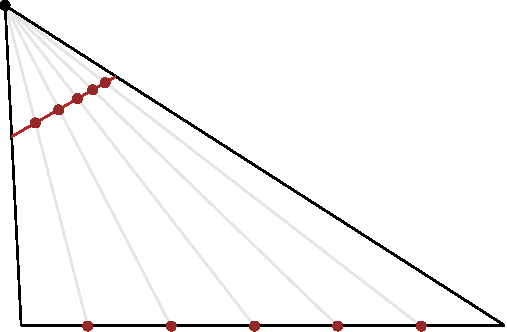
\includegraphics[scale=0.75]{figures/ProjectedGridVsWorldSpace.pdf}
\label{fig:subfigprojgrid1}
}
\subbottom[Projected Grid]
{
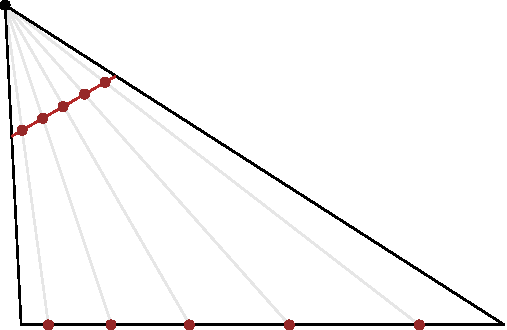
\includegraphics[scale=0.75]{figures/ProjectedGridUniform.pdf}
\label{fig:subfigprojgrid2}
}
\caption{The image on the left shows an uniform grid in worldspace,
its projection onto the image plane is not uniformly spaced though.
The image on the right on the other hand depicts an uniform grid on
the image plane and its associated non-uniform spaced worldspace
positions.}
\label{fig:projectedgrid}
\end{figure}

% The algorithm used for the projected grid can be broken down into the following
% steps:
% \begin{itemize}
%  \item create a uniformly spaced grid orthogonal to the viewer using normalised
% device coordinates
%  \item transform the grid to worldspace
%  \item project the grid onto the desired base plane
%  \item apply height displacement
%  \item run the grid through the rendering pipeline as usual
% \end{itemize}

\subsection{Coordinate Systems}
\label{sec:coordinate_systems}
Let $\mvec{x}$ be a vector representing the three dimensional carthesian
world space coordinate of a vertex, then
\begin{equation}
 \mvec{w} = \transpose{(\mvecx{x}, \mvecy{x}, \mvecz{x}, 1)}
\end{equation}
where $\mvec{w}$ is a homogeneous world space coordinate of $\mvec{x}$.
Let $\mmat{V}$ be the view matrix and $\mmat{P}$ the projection matrix, then
\begin{equation}
\label{eq:ws_to_cs}
 \mvec{c} = \mmat{P} \mmat{V} \mvec{w}
\end{equation}
where $\mvec{c}$ is the \textit{clip space} coordinate of $\mvec{w}$. For $\mvec{c}$ to
be inside the view frustum defined by $\mmat{P}$, $\mvec{c}$ is required to
meet the following condition
\begin{equation}
\label{eq:cs_bounds}
 \mvecx{c}, \mvecy{c}, \mvecz{c} \in \interval{-\mvecw{c}}{\mvecw{c}}
\end{equation}
where $\mvecw{c}$ is the homogeneous component of $\mvec{c}$. Next, clip space
vertex $\mvec{c}$ is transformed by the \textit{perspective division} as follows
\begin{equation}
\label{eq:cs_to_ndc}
 \mvec{n} = \frac{1}{\mvecw{c}}\transpose{(\mvecx{c}, \mvecy{c}, \mvecz{c})}
\end{equation}
where $\mvec{n}$ corresponds to the \textit{normalised device coordinate},
\textit{NDC} in short, of $\mvec{c}$.
%
%
\begin{figure}
\centering
\subbottom[View Frustum]
{
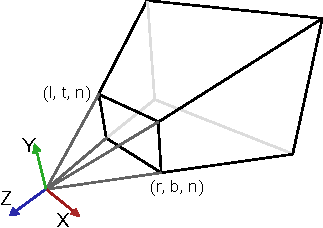
\includegraphics[width=0.4\textwidth]{figures/ProjectiveFrustum.pdf}
\label{fig:subfig_proj_frustum}
}
\subbottom[Canonical view volume]
{
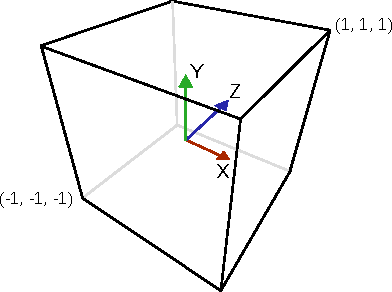
\includegraphics[width=0.4\textwidth]{figures/CanonicalCube.pdf}
\label{fig:subfig_canonical_view_volume}
}
\caption{Left: An example view frustum in view space. Right: The same view frustum
after applying projection and perspective division.}
\label{fig:proj_frustum_ndc}
\end{figure}
%
%
As one can see, equations~\ref{eq:cs_bounds}
and~\ref{eq:cs_to_ndc} imply
\begin{equation}
\label{eq:ndc_bounds}
 \mvecx{n}, \mvecy{n}, \mvecz{n} \in \interval{-1}{1}
\end{equation}
which defines the space NDC reside in, namely the \textit{canonical view volume},
see Figure~\ref{fig:proj_frustum_ndc}.\\


The projected grid, on the other hand, starts inside the canonical view volume
and needs to transform vertices back to world space. Let $\mvec{n}$ be the
normalised device coordinate of a vertex, then
\begin{equation}
\label{eq:ndc_to_cs}
 \mvec{c} = \transpose{(\mvecx{n}, \mvecy{n}, \mvecz{n}, 1)}
\end{equation}
where $\mvec{c}$ is a valid representation of $\mvec{n}$ in clip space. One may choose
a value for $\mvecw{c}$ different from $1$, making it necessary to scale $\mvecx{n}$,
$\mvecy{n}$ and $\mvecz{n}$ accordingly. Again, let $\mmat{V}$ be the view matrix and
$\mmat{P}$ the projection matrix, then
\begin{equation}
\label{eq:cs_to_wsh}
 \mvec{w} = \inverse{(\mmat{P} \mmat{V})} \mvec{c}
\end{equation}
where $\mvec{w}$ is a homogeneous world space coordinate of $\mvec{c}$. Conversion
to three dimensional carthesian world space is accomplished as follows
\begin{equation}
\label{eq:wsh_to_ws}
 \mvec{x} = \frac{1}{\mvecw{w}}\transpose{(\mvecx{w}, \mvecy{w}, \mvecz{w})}
\end{equation}

\subsection{Projection onto Plane}
As noted before, the vertices of the projected grid are represented as normalised
device coordinates. Assuming the plane the grid shall be projected on is specified
in world space coordinates, the following steps need to be computed for each vertex:
\begin{itemize}
 \item Transform vertex from canonical view volume to world space
 \item Setup vertex specific ray
 \item Intersect ray with target plane to compute actual position
\end{itemize}
Step one is already covered by Section~\ref{sec:coordinate_systems}. Step two
requires to setup a ray for each vertex, which implies both a position and a
direction. The position we already have, but to create a direction we need two
different positions. The solution is rather straightforward: let $\mvec{n}$ be
a \textit{two dimensional} vector representing the \textit{X} and \textit{Y}
components of a position in normalised device coordinates, then
\begin{align}
 \mvec{a} & = (\mvecx{n}, \mvecy{n}, -1, 1)\\
 \mvec{b} & = (\mvecx{n}, \mvecy{n}, +1, 1)
\end{align}
where $\mvec{a}$ corresponds to $\mvec{n}$ on the \textit{near plane} in clip space,
and $\mvec{b}$ to $\mvec{n}$ on the \textit{far plane} in clip space. Let $\mvec{d}$
and $\mvec{e}$ be the carthesian world space positions of $\mvec{a}$ and $\mvec{b}$
respectively, then
\begin{equation}
 \label{eq:proj_grid_ray}
 \mvec{p} = \mvec{d} + t(\mvec{e} - \mvec{d})
\end{equation}
where $\mvec{p}$ represents a ray starting at point $\mvec{d}$, pointing in direction
$(\mvec{e} - \mvec{d})$ with variable parameter $t$ controlling the actual position on
the ray.\\

Step three is about intersecting ray $\mvec{p}$ resulting from step two with the target plane.
We define the target plane using the \textit{Hesse normal form} as follows
\begin{equation}
\label{eq:proj_grid_plane}
 \mvec{p}\transpose{\mvec{n}} - d = 0
\end{equation}
where $\mvec{n}$ is the plane's normal vector with unit length and $d$ the plane's distance
from the origin. Next, we insert $\mvec{p}$ from equation~\ref{eq:proj_grid_ray}
into equation~\ref{eq:proj_grid_plane}, resulting in
%
\begin{gather}
\label{eq:plane_and_ray_intersection}
(\mvec{d} + t(\mvec{e} - \mvec{d})\transpose{\mvec{n}} - d = 0\\
\mvec{d}\transpose{\mvec{n}} + t(\mvec{e} - \mvec{d})\transpose{\mvec{n}} - d = 0\\
\intertext{solve for $t$}
t = \cfrac{d - \mvec{d}\transpose{\mvec{n}}}{(\mvec{e} - \mvec{d})\transpose{\mvec{n}}}
\end{gather}
%
where $t$ in combination with equation~\ref{eq:proj_grid_ray} gives the point of intersection
between the ray and the plane. In case $(\mvec{e} - \mvec{d})\transpose{\mvec{n}} = 0$,
there is no point of intersection because the ray is parallel to the plane.

\subsection{Projector}
\fxnote*{JÖSSAS}{Backfiring, etc}